\graphicspath{{images/act_3.1/}}
\subsection{PD control of end-effector pose}
The objective of this activity is to control pose (position and orientation) of the ur5 robot end-effector. The simulation starts with initial joint configuration $\mathbf{q_0}=\begin{bmatrix} 0.0 & -1.0 & 1.0 & 0.5 & 0.0 & 0.5 \end{bmatrix}$ rad and end-effector $\mathbf{p_0}=\begin{bmatrix}  0.577 &   0.192 &   0.364 \end{bmatrix}$~m. Therefore, desired Cartesian position is $\mathbf{p_0}$ and angle/axis orientation is  $\theta = \pi$ / $\mathbf{r}=\begin{bmatrix} 1 & 0 & 0 \end{bmatrix}$. Motion control is base on pose proportional-derivative method. Finally, control law can be computed as 
\begin{align}
	\boldsymbol{\tau} &= \mathbf{J^T} (\mathbf{W}^{d}), \label{eq:pose_PD}
	\\
	\mathbf{W}^{d} &=
	\begin{bmatrix}
	\mathbf{F}^{d} \\ \boldsymbol{\Gamma}^{d}
	\end{bmatrix}, 
	\nonumber \\
	\mathbf{F}^{d} &= \mathbf{\ddot{p}_{des}} + \mathbf{K_p (p_{des}-p)} + \mathbf{K_d (\dot{p}_{des}-\dot{p})}, 
	\nonumber \\
	\boldsymbol{\Gamma}^{d} &= \mathbf{\dot{w}_{des}} + \mathbf{K_o e_o} + \mathbf{D_o (\dot{w}_{des}-\dot{w})} \nonumber
\end{align}
\noindent where $\mathbf{J}$ is jacobian matrix, $\mathbf{p_{des}}$ is desired Cartesian position, $\mathbf{K_p, K_d}$ are Cartesian proportional and derivative gains respectively, $\mathbf{K_o, D_qo}$ are orientation proportional and derivative gains respectively, $\mathbf{w_{des}}$ is desired angular velocity and $\mathbf{e_o}$ is orientation error. \vspace{.5cm}






%\vspace*{0cm}
\begin{figure}%[H]
	\centering
	\subfloat[]{
	\includegraphics{ee_position_error.eps}
	}
	%\hfill
	\subfloat[]{
	\includegraphics{ee_velocity_error.eps}
	}	
	%\hfill
	\subfloat[]{
	\includegraphics{ee_acceleration_error.eps}
	}		
	\caption{Cartesian trajectory tracking error using pose proportional-derivative control method, \eqref{eq:pose_PD}, with  ${K_{p}}=1000$ $\mathrm{\frac{N}{m}}$, $K_{d}= 300$ $\mathrm{\frac{N.s}{m}}$, ${K_{o}}=800$ $\mathrm{\frac{N.m}{rad}}$, $K_{d}= 30$ $\mathrm{\frac{N.m.s}{rad}}$: (a) position, (b) velocity and (c) acceleration.}
	\label{fig:act_3.1_ee_position_error}
\end{figure}

\begin{figure}
    \centering
    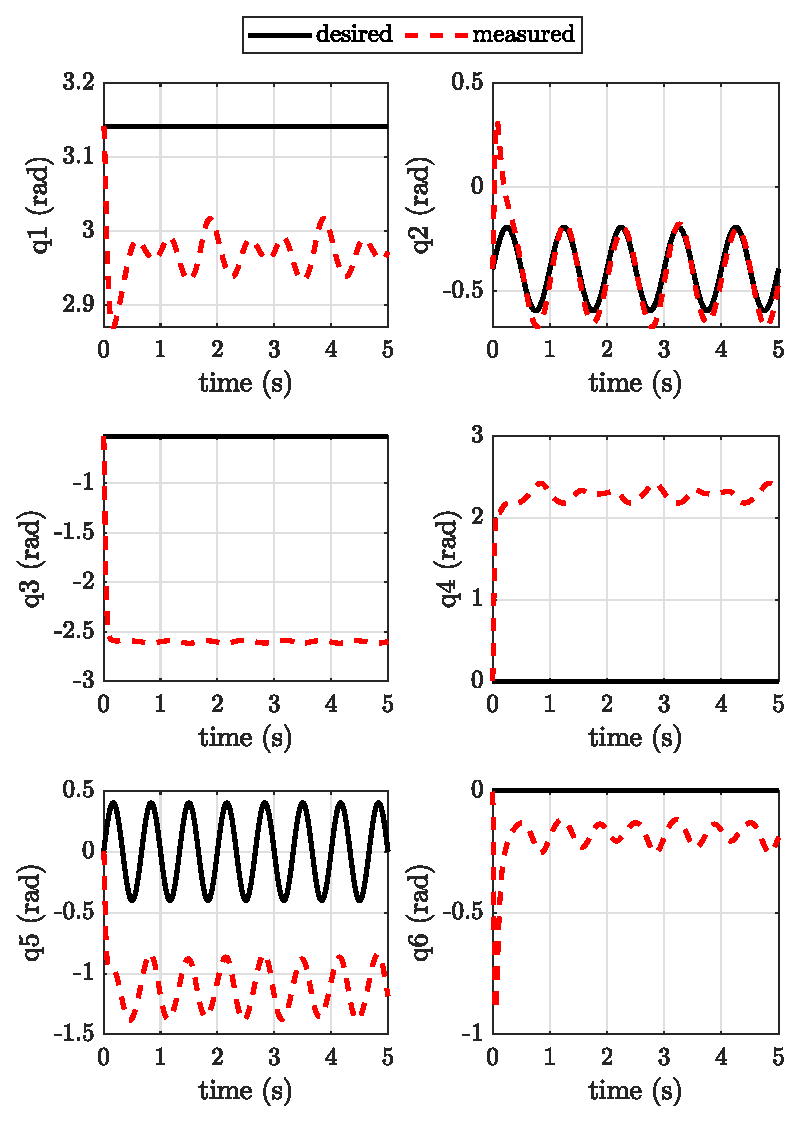
\includegraphics{joint_position.eps}	
    \caption{Angular position of each joint of UR5 robot with Algorithm \ref{lst:cartesian_idyn_N_simplified}.}
    \label{fig:act_3.1_joint_position_error}
\end{figure}